\documentclass[12pt]{beamer}
\usetheme{tau}
\usepackage{graphicx}
\graphicspath{{./fig/}}
\usepackage{pdfpages}
\usepackage{ulem}
\usepackage{tikz}

\newcommand{\fig}[1]{\centering\includegraphics[width=.95\textwidth,height=.7\textheight,keepaspectratio]{#1}}
\newcommand{\halffig}[1]{\includegraphics[width=.45\textwidth]{#1}}

\title[Uncertainty]{Uncertainty 101 (2nd week) }
\author{Engineering Testing and Measurements}
% \institute{School of Mechanical Engineering}
\date{}

\begin{document}

\begin{frame}
\titlepage
\end{frame}


\begin{frame}{Our main goal}

\textsc{\Large The science of good measurement}

\vspace{3cm}

\textbf{Good == accurate, low uncertainty}

Uncertainty is: \alert{``a quantitative estimate of the possible range of all the errors in the measurement''} 

\end{frame}


\begin{frame}{Measurement error is only a small part of uncertainty}
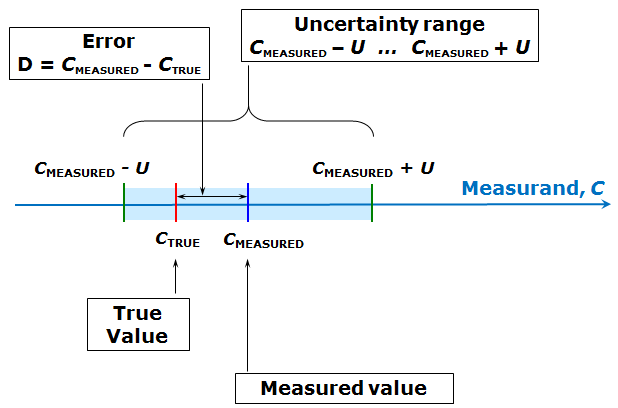
\includegraphics[width=.9\textwidth]{error_vs_uncertainty_2}
%\small{\url{https://www.engineering.com/story/an-introduction-to-metrology-and-quality-in-manufacturing}}
\end{frame}

%
%\begin{frame}{Uncertainty}
%
%\alert{The uncertainty is a quantitative estimate of the possible range of all the errors in the measurement - it is a concept and it relates only to the result of the measurement}
%
%\begin{itemize}
%\item \textbf{All of the errors}:  --  \textbf{calibration}, the data
%set \textbf{statistics}, and the \textbf{measurements}. 
%
%\item Individual errors are properties of the \textbf{instruments},
%the \textbf{test method}, the \textbf{analysis}, and the \textbf{measurement
%system}. 
%
%\end{itemize}
%\end{frame}



%\begin{frame}
%\begin{enumerate}
%\item What question are we trying to answer? (What is the problem?) 
%\item How accurately do we need to know the answer? (How is the answer to
%be used?) 
%\item What physical principles are involved? (What physical laws govern
%the situation?) 
%\item What experiment or set of experiments might provide the answer? 
%\item What variables must be controlled? How well? 
%\item What quantities must be measured? How accurately? 
%\item What instrumentation is to be used? 
%\item How are the data to be acquired, conditioned, and stored? 
%\item How many data points must be taken? In what order? 
%\item Can the requirements be satisfied within the budget and time constraints? 
%\item What techniques of data analysis should be used? 
%\item What is the most effective and revealing way to present the data? 
%\item What unanticipated questions are raised by the data? 
%\item In what manner should the data and results be reported?
%\end{enumerate}
%\end{frame}
%
\begin{frame}{Why uncertainty is \textbf{crucial} for engineers}

\small{We work with a concept or ``model of reality'', we need measurements to decide which model fits best:}
%
\fig{two_models_experiment}
%

\end{frame}
%
\begin{frame}{Can we take a decision with this uncertainty level?}
	\fig{two_models_uncertainty}
\end{frame}
%
%\begin{frame}{If you do it professionally, learn it}
%	\fig{book_uncertainty}
%\end{frame}
%
\begin{frame}{Conceptual picture }
	\fig{uncertainty_concept}
\end{frame}
%
%\begin{frame}{Uncertainty is a ``distance from a true value''}
%	\fig{temperature_with_bias}
%\end{frame}
%
%% From errors_resolution.tex

\begin{frame}[plain]{Errors}

\alert{systematic} (or \textbf{bias}) errors and \alert{random} (or \textbf{precision})
errors. 


\begin{description}
\item [{Systematic}] \textbf{(bias) errors} are consistent, repeatable
errors. example: old ruler without a first 2 mm (also called zero
error)
\item [{Random}] \textbf{(precision) errors} caused by a \textbf{lack of
repeatability} in the output of the measuring system, e.g. \textbf{scatter}
in the measured data. For example, background electrical \textbf{noise}
often results in small \textbf{random errors} in the measured output. 
\end{description}
\end{frame}

\begin{frame}
	\fig{random_systematic_error}
\end{frame}

\begin{frame}{Systematic error, bias}

\begin{itemize}
\item Consistent, repeatable errors defined as the
\textbf{average of measured values minus the true value}, $\overline{x_{i}-x_{\mathrm{true}}}$. 
\item Reasons: 
\begin{itemize}
\item {\bf calibration errors } -- inherent, see lecture on calibration 
\item loading or intrusive errors -- the sensor may actually change the very
thing it is trying to measure. 
\item spatial errors -- when a quantity varies in space, but a measurement
is taken only at one location (e.g. temperature in a room). 
\item human errors -- these can arise if a person consistently reads a scale
on the low side
\item defective use of equipment --  some internal problem or damage, lack of calibration 
\end{itemize}
%\item A non-dimensional form of bias error is the \textbf{mean bias error},
%defined as \textbf{MBE = systematic error / true value}. 
\end{itemize}
\end{frame}

%\begin{frame}{Random errors, precision}
%
%Unrepeatable, inconsistent errors in the measurements, scatter in the data. 
%
%\begin{itemize}
%\item The \textbf{random error} of one data point $x_{i}$ is defined as
%the reading minus the \textbf{average of data}, $x_{i}-\overline{x}$
%
%\begin{itemize}
%\item Five temperature readings: -1.30, -1.50, -1.20, -1.60, and -1.50 $^{\circ}C$.
%\item Find the \textbf{maximum magnitude of random error} in $^{\circ}C$. 
%\item Average $\overline{x} =  -1.42^{\circ}$C. 
%\item The largest deviation is  $-1.20 - (-1.42) = 0.22^{\circ}$C.
%\item \textbf{maximum absolute value of random error} is 0.22$^{\circ}C$. 
%\end{itemize}
%\end{itemize}
%\end{frame}

%\begin{frame}{Accuracy}
%
%\begin{itemize}
%\item \textbf{Accuracy} is the \textbf{closeness of agreement between a
%measured value and the true value, $x_{i}-x_{\mathrm{true}}$} 
%\item The accuracy error of a reading is \textbf{a combination of bias
%and precision errors} 
%\item The \textbf{overall accuracy} \textbf{error} (or the \textbf{overall
%inaccuracy}) of a set of readings is defined as the \textbf{average
%of all readings minus the true value}. 
%\end{itemize}
%\end{frame}

%\begin{frame}{Example }
%
%\begin{itemize}
%\item Temperature readings: -1.30, -1.50, -1.20, -1.60, and -1.50$^{\circ}C$. 
%\item Known that the true temperature is -1.45$^{\circ}C$. 
%\item To do: Calculate the accuracy error of the third data point in $^{\circ}C$.
%What is the overall accuracy error? 
%\item Solution: The accuracy error (that is, the inaccuracy) of this data
%point is defined as the reading minus the true value, or -1.20 - (-1.45)
%= 0.25$^{\circ}C$. 
%\item The overall accuracy error is the same as the systematic error or
%bias error, which is the average reading minus the true value, i.e.,
%-1.42 - (-1.45) = 0.03$^{\circ}C$. 
%\end{itemize}
%\end{frame}

%\begin{frame}{Precision}
%
%\begin{itemize}
%\item \textbf{Precision} \textbf{characterizes the random error} of the
%instrument output 
%\item \textbf{Precision error} (of one reading) is defined as the \textbf{reading
%minus the average of readings}. 
%\item Thus, \textbf{precision error} \textbf{is identical to random error}
%\item Instrument precision related to instrument resolution, but these are
%not the same thing. An instrument can have great resolution, but poor
%precision. 
%\end{itemize}
%\end{frame}

%\begin{frame}{Precise or accurate?}
%
%Both random and systematic errors affect accuracy.
%
%\begin{center}
%\includegraphics[width=1\textwidth]{figures/darts}
%\par\end{center}
%\begin{itemize}
%\item It is proper to say: (a) is more precise than (c), but not as accurate.
%On the other hand, (c) is more accurate than (a), but not as precise.
%(b) is Robin Hood's result
%\item Instrument precision related to instrument resolution, but these are
%not the same thing. An instrument can have great resolution, but poor
%precision. 
%\end{itemize}
%\end{frame}

\begin{frame}{Resolution}


\begin{description}
\item [\alert{Resolution}] the smallest change or increment in the measured quantity
that the instrument can detect. 
\end{description}


Characterizes the \textbf{ability} of instrument 
\textbf{output} to show \textbf{changes in the quantity}.  

\begin{itemize}
\item Digital instruments, resolution is the number of digits displayed on the output.
\end{itemize}
A {\bf high resolution} instrument is \alert{neither precise nor accurate}
\end{frame}

\begin{frame}{True time is 45.67 s}

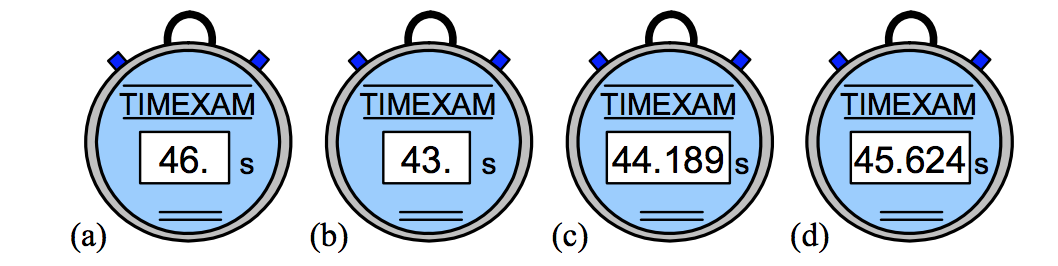
\includegraphics[width=1\textwidth]{stopwatchexample}

\bigskip

(a) ............... (b) ................. (c) ................ (d) ..................

\end{frame}

\begin{frame}
(a) poor resolution (1 sec) but best possible job (compare to c), accurate
if rounded time is considered

(b) poor resolution, inaccurate.

(c) very good resolution, very inaccurate

(d) good resolution, most accurate
\end{frame}



\begin{frame}{Uncertainty combines all the sources }

Root-of-the-sum-of-the-squares combines \textbf{precision}
uncertainty, \textbf{bias} uncertainty: 

\[
u_{x}=\sqrt{\left(u_{\textrm{systematic}}\right)^{2}+\left(u_{\textrm{random }}\right)^{2}}=\sqrt{\sum u_{b_i}^{2}+\sum u_{p_i}^{2}}
\]

\end{frame}


%\begin{frame}{Example}
%
%Rotation speed of a shaft has been measured by stroboscope with many
%repetitions. $\overline{N}=1734.2$ rpm, $S_{N}=1.45$ rpm. 
%
%\begin{itemize} 
%\item Bias, systematic error:
%\begin{itemize}
%	\item Strobe accuracy is given by manufacturer $\pm1.00$rpm (assumed to
%be 95\% confidence level), $u_{\textrm{b}}=\pm 1.00$ rpm
%\end{itemize}
%\item Combine with the standard uncertainty for 95\%
%$$u_{N}=\sqrt{u_{\textrm{p}}^{2}+u_{\textrm{b}}^{2}}=\sqrt{2.90^{2}+1.00^{2}}=3.068\, \mathrm{rpm}$$ 
%
%$$
%	N=1734.2 \pm 3.07\,\textrm{rpm}
%$$ 
% (with 95\% confidence level) 
%
%\end{itemize}
%\end{frame}

% \includepdf[pages=36-47]{uncertainty101}

\begin{frame}
\frametitle{Eight steps to get the correct measurement}

\fig{8steps}

\end{frame}
%
%\begin{frame}
%\frametitle{ This is just the simplest case }
%
%This is a simple example, we do not deal with special cases where different rules apply such as:
%
%\begin{itemize}
%\item Small number of repeated readings -- ``Student'' distribution
%\item If one aspect of uncertainty dominates the calculation 
%\item If the inputs to the calculation are correlated
%\end{itemize}
%\end{frame}


%
\begin{frame}{Combination of uncertainties}
\begin{itemize}
\item We measured $N$ physical quantities (variables), $x_{1},x_{2},\ldots,x_{N}$
(voltage, resistance, power, torque, length), each has its own uncertainty,
$u_{x_{i}}$ (component uncertainty): 
\[
x_{i}=\overline{x_{i}}+u_{x_{i}}
\]
\item We want to estimate uncertainty of the result $R$ that depends on
the measured ones: $y=f(x_{1},x_{2},\ldots,x_{N})$. 
\item We need to estimate $u_{y}$, using $u_{x_{i}}$ to obtain:
\[
y=\overline{y}\pm u_{y}
\]
\item \textbf{Two} \textbf{types}: \alert{maximum} (worst case) or \alert{expected}
(probabilistic)
\end{itemize}
\end{frame}

%
\begin{frame}{Theory of uncertainty analysis }
{\large  Taylor expansion}

\[
y + u_y = f(x_1 + u_{x_1}, x_2 + u_{x+2}, ... )  = 
\]

\[
= f(x_1, x_2 , ...) + \frac{\partial f}{\partial x_1} u_{x_1} +  \frac{\partial f}{\partial x_2} u_{x_2} + ...  + 
\]


\[
+ \frac{1}{2} \left( (u_{x_1} )^2 \frac{\partial^2 f}{\partial x_1^2} +  ...   \right)
\]

\end{frame}


%
\begin{frame}{Maximum uncertainty}

\[
u_{y,\mathrm{max}}=\sum_{i=1}^{i=N}\left|u_{x_{i}}\frac{\partial y}{\partial x_{i}}\right|
\]
\begin{itemize}
\item We assume that all the errors in the component measurements will \textbf{ADD}
to the uncertainty of $R$, i.e. will be always of the same sign. 
\item This is worst case scenario, unlikely for large number of variables
(large $N$), but happens when we have a direct effect or a bias error
(broken ruler, wrong diameter of spheres in cone measurements, lab
A)
\end{itemize}
\end{frame}

\begin{frame}{Expected uncertainty}

Root of the sum of squared uncertainty, RSS:

\[
u_{R,\mathrm{RSS}}=\sqrt{\sum_{i=1}^{i=N}\left(u_{x_{i}}\frac{\partial R}{\partial x_{i}}\right)^{2}}
\]
\begin{itemize}
\item More realistic for large number of variables or for very different
variables (using different instruments, randomization)

\item ISO standard if not stated otherwise:  $ u_{R}=u_{R,\textrm{RSS}}$ 

\item We known that $R=\overline{R}+u_{R}$ at the same confidence level
as the components, typically 95\% confidence level

\item Use dimensionless $u_{R}/R$
\end{itemize}
\end{frame}


\begin{frame}{Example}

Combining uncertainty for the measurement of a bolt using calipers


\fig{calipers_bolt}

\small{\url{https://www.muelaner.com/uncertainty-budget/}}
\end{frame}


\begin{frame}
\frametitle{8 steps plan}


\begin{center}
        \begin{tikzpicture}
            \node[anchor=south west,inner sep=0] (image) at (0,0) {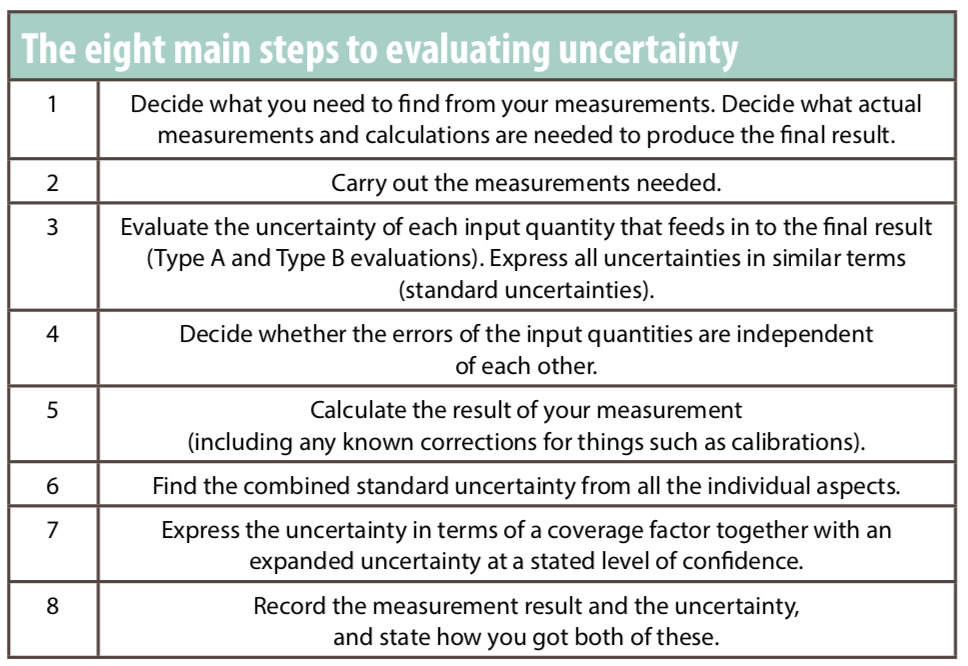
\includegraphics[width=1\textheight]{8steps}};
            \node[align=center, xshift=0mm, yshift=15mm,red,font={\Large\bfseries}] at (image.center) {From step 3 to 8 };
        \end{tikzpicture}
    \end{center}
    
    
% \fig{8steps}

\end{frame}

\begin{frame}{List sources of uncertainty}

\begin{itemize} 
\item Calibration ($x_\mathrm{cal}$) error in mm; 
\item Resolution ($x_\mathrm{res}$) error in mm; 
\item Cosine Error ($x_{\cos}$) angular misalignment; 
\item Temperature ($x_T$) error in degrees C; 
\item Repeatability ($x_\mathrm{rep}$) error in mm. 

%The measurement result ($y$) is a function of these uncertainties as well as the actual length of the measurand ($Y$). 

%Unlike in previous examples the input quantities have different functional relationships with the measurement result. The functional relationship between these quantities can be written.

\end{itemize}

\[ 
y = Y + x_\mathrm{cal} +x_\mathrm{res} +Y \left( 1 - \cos \left( x_{\cos} \right) \right) + Y  x_{T} \frac{\partial x}{\partial T} + x_\mathrm{rep}
\]

\end{frame}


\begin{frame}{Simplest case}

Simplest case is when all sources are: a) same units, b) all normally distributed: $\Delta y = x_1 + x_2 + \ldots + x_n$

\fig{uncertainty-budget-1b.png}

\end{frame}


\begin{frame}{When distributions are different}

\fig{central-limit-theorem.png}
\end{frame}

\begin{frame}{We have to consider different contributions}

For each input uncertainty the units of measurement and probability distribution must first be stated. A divisor is used to account for the way that different probability distributions contribute different amounts to the combined uncertainty. A sensitivity coefficient is used to adjust the input value for different units of measurement and for the way in which it contributes to the combined uncertainty.

\end{frame}

\begin{frame}

Nominal length = 100 mm, bolt material Aluminium with CTE=23ppm


\fig{full-uncertainty-budget}
\end{frame}

\begin{frame}{Type A uncertainties}
\begin{itemize}
\item Uncertainties which are determined through repeated measurements are called Type A, they are generally assumed to follow a normal distribution.
\item Calibration uncertainty is also assumed to be a normal distribution and is simply divided by the coverage factor for the given level of confidence.
\item For example if a 95\% confidence level calibration uncertainty is given then it is divided by the coverage factor 2.
\item We will study calibrations (static, dynamic) later in the course
\end{itemize}
  
\end{frame}

\begin{frame}{Type B uncertainties}
\begin{itemize}
%\item Uncertainties obtained from other means such as estimates or specifications are called Type B
\item Follow a rectangular distribution especially where hard limits are given for an input quantity or little other information is available.
\item A rectangular distribution: zero probability of the value outside of the limits and an equal probability of having any value within the range ($ \pm a$)
\item Two rectangular distributions with limits of $\pm a$ combine to give a triangular distribution of $\pm 2a$.
\item Three and more going to $t$ distribution for small number of samples (later in the course)
\item  $U$-shaped distributions are sometimes encountered in electronics. 
\end{itemize}
\end{frame}

\begin{frame}
\fig{Distributions-and-Divisors}
\end{frame}

\begin{frame}{Sensitivity coefficients}
Sensitivity coefficients allow us to add sources together which have different units of measurement and/or different functional relationships



In the GUM this is given in the form of a partial differential equation, the partial differentials simply describe the rate at which the measurement result will change if one of the input quantities changes. 



Since we generally know the approximate value of the measurement result we can simply calculate a sensitivity coefficient ci in place of these terms which gives the ratio for change in the measurement result per unit change in the input.

\[
y + u_y = f(x_1 + u_{x_1}, x_2 + u_{x+2}, ... )  = 
\]

\[
= f(x_1, x_2 , ...) + \frac{\partial f}{\partial x_1} u_{x_1} +  \frac{\partial f}{\partial x_2} u_{x_2} + ...  + 
\]


\[
+ \frac{1}{2} \left( (u_{x_1} )^2 \frac{\partial^2 f}{\partial x_1^2} +  ...   \right)
\]

\end{frame}

\begin{frame}{Approximate linear relation}

Simplifying the equations also means that we can multiply the uncertainty in the input by the sensitivity coefficient before squaring

\[ \frac{\partial f}{\partial x_i} \approx \frac{\Delta f}{\Delta x_i} \approx c_i \]

in the RSS method:

\[ u_c^2(y) = \sum\limits_{i=1}^{N} \left( \frac{\partial f}{\partial x_i} \right)^2 u^2(x_i) \]

\[ u_c^2(y) \approx \sum\limits_{i=1}^{N} c_i^2 u^2(x_i) = \sum\limits_{i=1}^{N} (c_i u(x_i))^2 \]

\end{frame}


\begin{frame}{Example of simplifying sensitivity coefficient}
\fig{Clinometer-Measurement-of-Flag-Pole}
\end{frame}

\begin{frame}{Simplification of sensitivity coefficient}

\[ H = d \tan(\phi) \]

$ d = 10$m $\pm 0.1$ m, $\phi = 27^\circ \pm 0.1^\circ$

\[ H = 10 \tan(27^\circ) = 5.095 \mathrm{m} \]

Instead of $c_d = \partial H/\partial d$ we can use extreme values: $d = 10.1 \to H = 5.146$, $d=9.9 \to H=5.044$. Simple estimate $c_d = \Delta H/\Delta d = 0.5095$ 

Similarly for $\phi$: $\phi = 27.1^\circ \to H = 5.117 \to \Delta H/\Delta \phi = 0.2200$, $\phi = 26.9^\circ \to H = 5.073 \to \Delta H/\Delta \phi = 0.2196$. When the value is not constant, use the extreme case to be on the safe side, $c_\phi \approx 0.22$. 

\end{frame}

\begin{frame}{Special case - misalignment}
\fig{cosine-sensitivity-combined}
\end{frame}

\begin{frame}{Misalignment sensitivity}
Obviously it's wrong: $\partial L/\partial \theta = 0$, as it says misalignment does not contribute to the uncertainty. 

The practice is to use extreme values in the range, e.g. for nominal length of 100 mm, an angular error of $\pm 3^\circ$ can result in $100 \times (1-\cos 3^\circ ) = 0.137$ mm. Thus:

\[ \Delta L/\Delta \theta = 0.137/3^\circ \approx 0.046 \mathrm{mm}/^\circ \] 

\end{frame}


\begin{frame}{Thermal expansion}

\[ \Delta L = \Delta T \alpha L \]

\[\Delta L/\Delta T = L\, \alpha \]

For example, for a 100 mm aluminium bolt with CHT=23 ppm it's $\alpha = 23 \times 10^{-6}$ K$^{-1}$, thus:

\[c_T = 0.0023 \mathrm{mm}/^\circ C\]

\end{frame}


\begin{frame}{Calculating Standard Uncertainties}
\begin{enumerate}
\item Each source is divided by its divisor and multiplied by its sensitivity coefficient to give \alert{standard uncertainty}

\item  We emphasize it by changing $u(x_i)$ to $u_i(y)$ - because now we are with the same units of the property we measure

\end{enumerate}

\end{frame}


\begin{frame}{Calculating the Combined Standard Uncertainty}

Maximum uncertainty: 

\[
u_{y,\mathrm{max}}=\sum_{i=1}^{i=N}\left|u_{x_{i}}\frac{\partial y}{\partial x_{i}}\right|
\]

or the square root of the sum of each standard uncertainty squared (RSS):

\[
u_{R,\mathrm{RSS}}=\sqrt{\sum_{i=1}^{i=N}\left(u_{x_{i}}\frac{\partial R}{\partial x_{i}}\right)^{2}}
\]

\end{frame}


\begin{frame}{Using a Coverage Factor to Calculate the Expanded Uncertainty}

\begin{enumerate}
\item Since the combined uncertainty has a normal distribution we have only 68\% confidence that the true value lies within $\pm$ the combined standard uncertainty $u_c(y)$ of the measurement result. 

\item It is therefore standard practice to multiply the combined standard uncertainty by a coverage factor ($k$) to give the \alert{Expanded Uncertainty} ($U$). 
\end{enumerate}
\end{frame}

\begin{frame}{Result}
\fig{Calculating-Combined-Standard-Uncertainty}
\end{frame}
%
\begin{frame}{Standard uncertainties}

\[ L = 100 \pm 0.165 \mathrm(mm) (95\%) \]

\fig{Calculating-standard-uncertainties-with-budget}

%We have now covered all the steps involved in creating a full uncertainty budget for a measurement process or calibration.

\end{frame}

\begin{frame}{Maybe we need to change our decision?}

Note the result of careful uncertainty budget is larger than the simplest case estimate - \alert{do we have to change our decision?}

\fig{two_models_uncertainty}

\end{frame}

\\
\begin{frame}{Uncertainty analysis helps to manage your budget}

\begin{itemize}
\item Shaft rotation speed measured by stroboscope with many
repetitions. $\overline{N}=1734.2$ rpm, $S_{N}=1.45$ rpm. 
\item Strobe accuracy by manufacturer $\pm 1.00$ rpm
\item $u_{\textrm{measurement}}=\pm 2\sigma=\pm 2.90$ rpm (95\%)
$u_{\textrm{instrument}}=\pm1.00$ rpm 
\item $u_{N}=\sqrt{u_{\textrm{meas.}}^{2}+u_{\textrm{instr.}}^{2}}=\sqrt{2.90^{2}+1.00^{2}}=3.068$ rpm 
\item The final result is:
\[
N=1734.2\pm3.07\,\textrm{rpm} (95\% \mathrm{c.l.})
\]
\item The uncertainty is due to {\bf the measurement uncertainty},
thus a more expensive tool will not help. 
\end{itemize}
\end{frame}



\end{document}